\chapter{Résultat}
\begin{spacing}{1.2}
\minitoc
\thispagestyle{MyStyle}
\end{spacing}
\newpage

\section{INTRODUCTION}
 Dans ce chapitre, nous planifierons la première version de notre projet en la répartissant en 2 sprints. Nous nous concentrerons sur les « user stories » pour chaque sprint afin de produire des incréments livrables. Nous aborderons également la phase d'analyse et les solutions conceptuelles en utilisant divers diagrammes pour illustrer les interactions entre les systèmes et les utilisateurs.
\section{Sprint 1: S'inscrire, s'authentifier et créer des formulaires}
\subsection{ Analyse des besoins}
\subsubsection{Diagramme de cas d'utilisation du Sprint 1}
Le diagramme de cas d'utilisation du Sprint 1 illustre les interactions entre les utilisateurs (administrateurs et utilisateurs) et le système.
\begin{figure}[H]
    \centering
    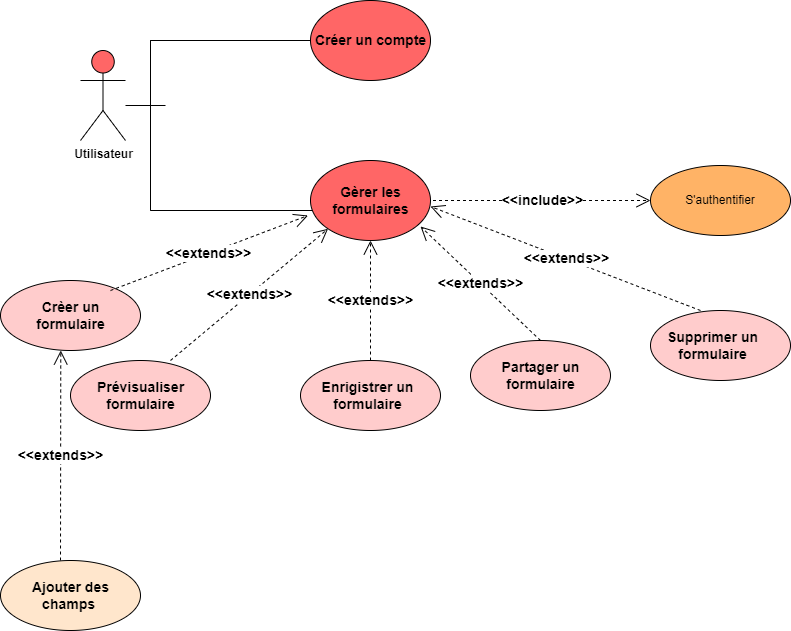
\includegraphics[width=0.8\textwidth]{images/release1.drawio.png}
    \caption{Diagramme de cas d’utilisation du Sprint 1}
\end{figure}
\subsubsection{Diagramme de classe du Sprint 1}
\section{ Interfaces liées à un utilisateur}
\subsection{Interface : S’inscrire}
 Grâce à la page d’inscription, les utilisateurs peuvent créer un compte afin de pouvoir
 bénéficier de nos services
\begin{figure}[H]
    \centering
    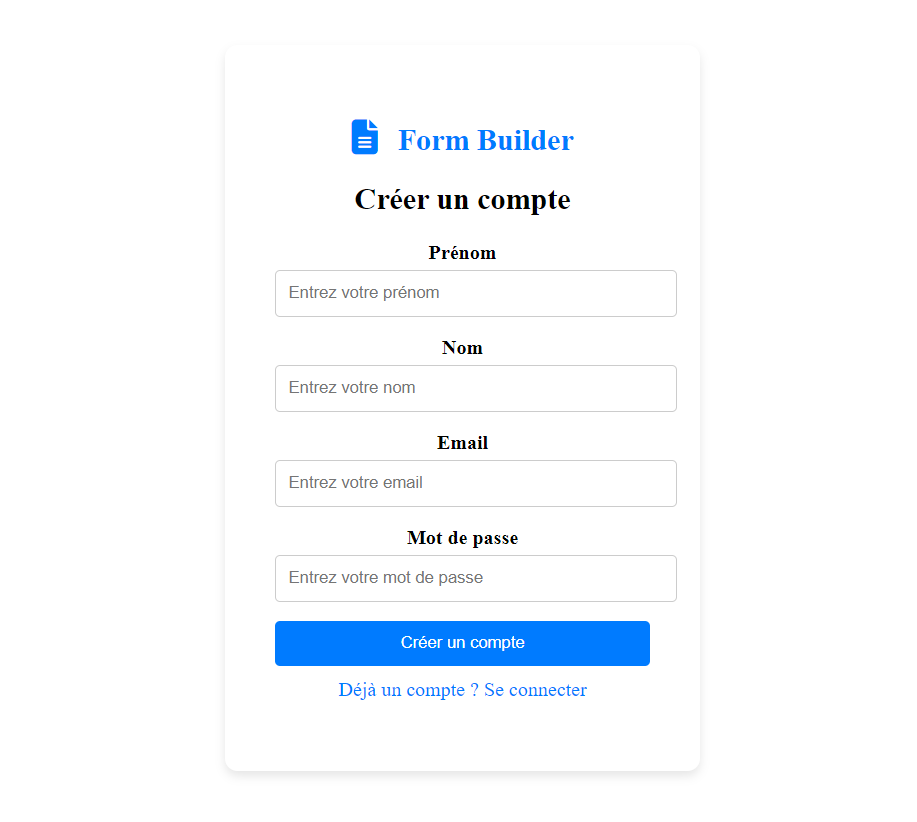
\includegraphics[width=1.1\textwidth]{images/S'inscrire.png}
    \caption{Page d’inscription}
\end{figure}
\subsection{Interface : S’Authentifier}
\begin{figure}[H]
    \centering
    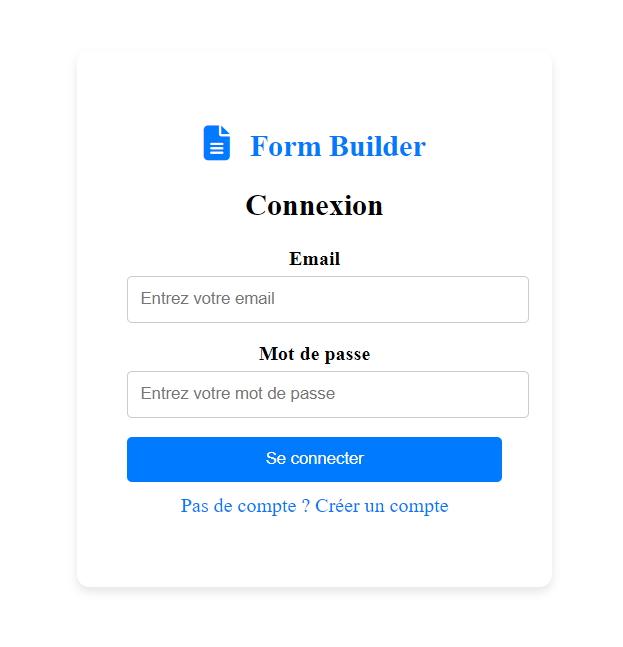
\includegraphics[width=0.8\textwidth]{images/S'authentifier.png}
    \caption{Page d’authentification}
\end{figure}
\subsection{Interface : Créer un nouveau formulaire}
\begin{figure}[H]
    \centering
    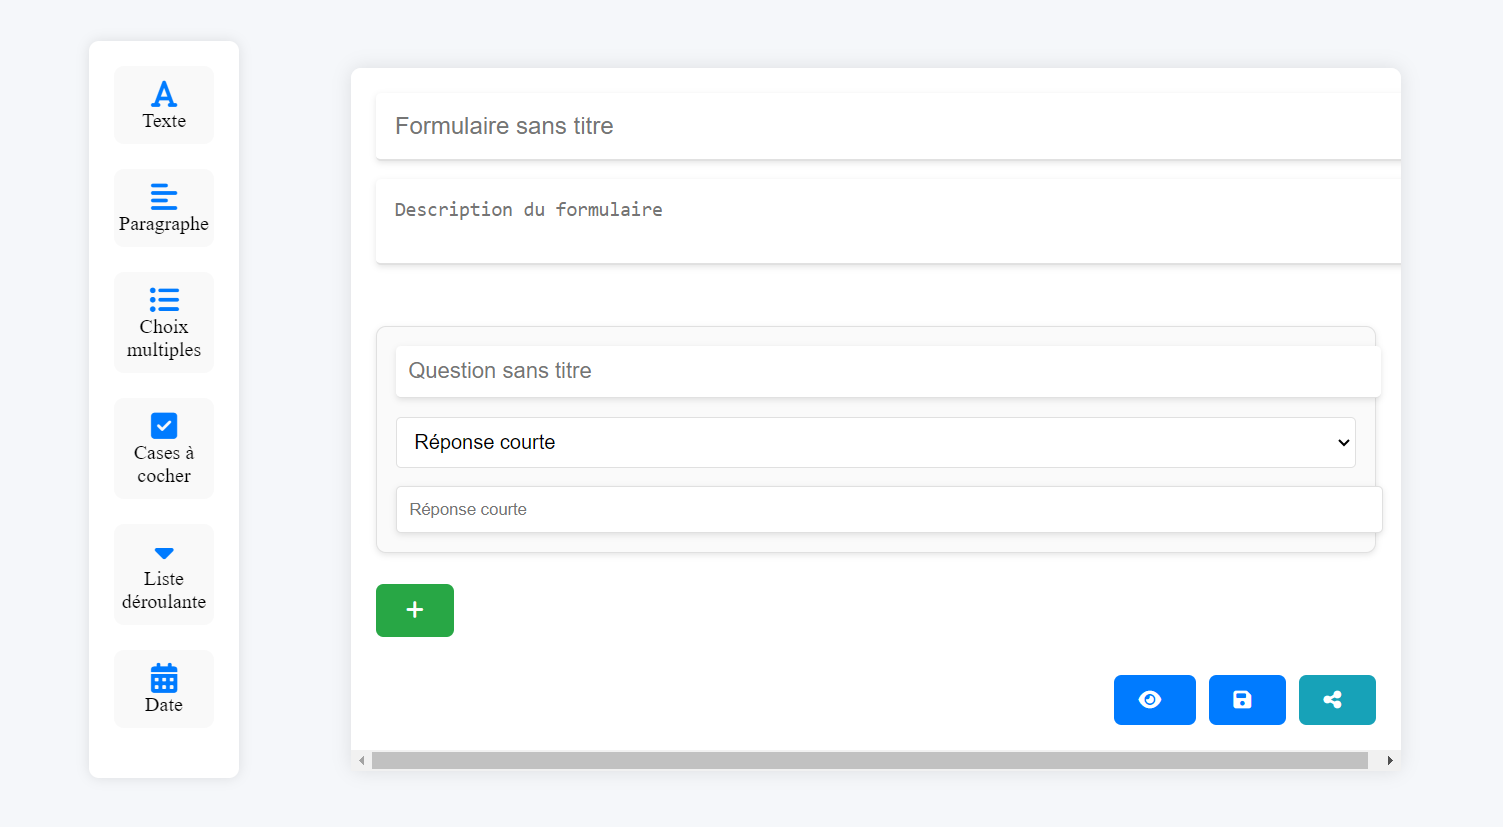
\includegraphics[width=1.0\textwidth]{images/Creer.png}
    \caption{Page de création du formulaire}
\end{figure}
\section{ Conclusion}
Ce chapitre se focalise sur la finalisation du sprint 1, une étape cruciale dans notre processus de développement. Nous avons pris le soin de créer des diagrammes détaillés qui illustrent les interactions complexes entre les divers composants du système. Simultanément, nous avons intégré les interfaces de la plateforme, en alignant la conception avec les exigences fonctionnelles. Cette approche rigoureuse nous a permis de fournir une vue complète de la conception et de poser une base solide pour les étapes suivantes du projet.


